\begin{song}{title=\centering Zatanči \\\normalsize Jaromír Nohavica  \vspace*{-0.3cm}}  %% sem se napíše jméno songu a autor
\moveright \stred \vbox{      %Varianta č. 1  ---> Jeden sloupec zarovnaný na střed	

\sloka
^{Emi G}Zatanči, má milá, ^{D}zatanči ^{Emi}pro mé oči,

^{G}zatanči a vetkni ^{D}nůž do mých ^{Emi}zad,

ať tvůj ^{G}šat, má milá, ^{D}ať tvůj šat ^{Emi}na zemi skončí,

ať tvůj ^{G}šat, má milá, ^{D}rázem je ^{Emi}sňat.

\refren
^{Emi G}Zatanči, jako se ^{D}okolo ^{Emi}ohně tančí,

^{G}zatanči jako ^{D}navodě ^{Emi}loď,

^{G}zatanči jako to ^{D}slunce mezi ^{Emi}pomeranči,

^{G}zatanči, a ^{D}pak ke mně ^{Emi}pojď.

\sloka
Polož dlaň, má milá, polož dlaň na má prsa,

polož dlaň nestoudně na moji hruď,

obejmi, má milá, obejmi moje bedra,

obejmi je pevně a mojí buď.

\refren

\sloka
Nový den než začne, má milá, nežli začne,

nový den než začne, nasyť můj hlad,

zatanči, má milá, pro moje oči lačné,

zatanči a já budu ti hrát.

\refren

\refren
}
\setcounter{Slokočet}{0}
\end{song}

\begin{figure}[h]
\centering
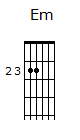
\includegraphics[scale=1.5]{../Akordy/em.png} 
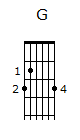
\includegraphics[scale=1.5]{../Akordy/g.png}
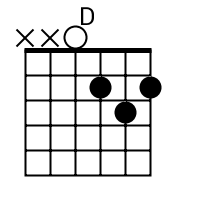
\includegraphics[scale=1.5]{../Akordy/d.png}
\end{figure}